\documentclass[ignorenonframetext, aspectratio=169]{beamer}

\title{Trump \textit{v.}\ United States}
\subtitle{Presidental immunity and the separation of powers}
\author{Runxi Yu}
\date{August 10, 2024}

\usetheme{Hannover}

\usepackage{tgschola}
\usepackage{tgheros}
% \usepackage{tgcursor}
\usefonttheme{professionalfonts}
\renewcommand{\familydefault}{\rmdefault}
\usepackage{microtype}

\usepackage[notes, backend=biber, useibid=true]{biblatex-chicago} % remove noibid when fixed capitalization
\addbibresource{/home/runxiyu/phil/db.bib}
\newcommand{\nopage}{\_\_\_\_}
\newrobustcmd*{\Runcite}{\bibsentence\runcite}

\usepackage{graphicx}

\hypersetup{
	colorlinks=false,
}

\begin{document}

\begin{frame}
\titlepage
\end{frame}

\begin{frame}[fragile]{Miscellaneous information}
\begin{itemize}
	\item Except for text included within double quotation marks and text within a \verb|quote|/\verb|quotation| environment, all text in this slide show is in the public domain, available under Creative Common Zero version 1.0, or the 0-clause BSD license, at your option.
	\item This does not mean that the entire slide show (especially images) is public domain. However, quotes of court opinions are public domain; see 17 U.\,S.\,C.\ {\S} 105 and \Runcite{banks}.
	\item The source code of this slide show is available in \href{https://git.sr.ht/~runxiyu/philo}{\texttt{https://git.sr.ht/\~{}runxiyu/philo}}. Tarballs and rsync may be provided on-demand.
	\item This slide show uses \texttt{biblatex-chicago} for SCOTUS-style citations, which are generally of the form ``\textit{Petitioner} v.\ \textit{Respondent}, Volume U.\,S. Start-page, Page (Year)''.
\end{itemize}
\end{frame}

\section{Background}

\begin{frame}{What is Trump \textit{v.}\ United States?}
\begin{itemize}
	\item \href{https://www.supremecourt.gov/docket/docketfiles/html/public/23-939.html}{SCOTUS docket 23--939}
	\item Donald Trump was prosecuted for the January 6th riot
	\item ``The indictment alleged that after losing that election, Trump conspired to overturn it by spreading knowingly false claims of election fraud to obstruct the collecting, counting, and certifying of the election results.'' \Runcite[\nopage{} (slip op., at 1)]{tvus}
	\item The district and circuit courts ruled against Trump, so he appealed to the Supreme Court.
\end{itemize}
\end{frame}

\begin{frame}{What happened on January 6th 2021?}
\begin{figure}
	\centering
	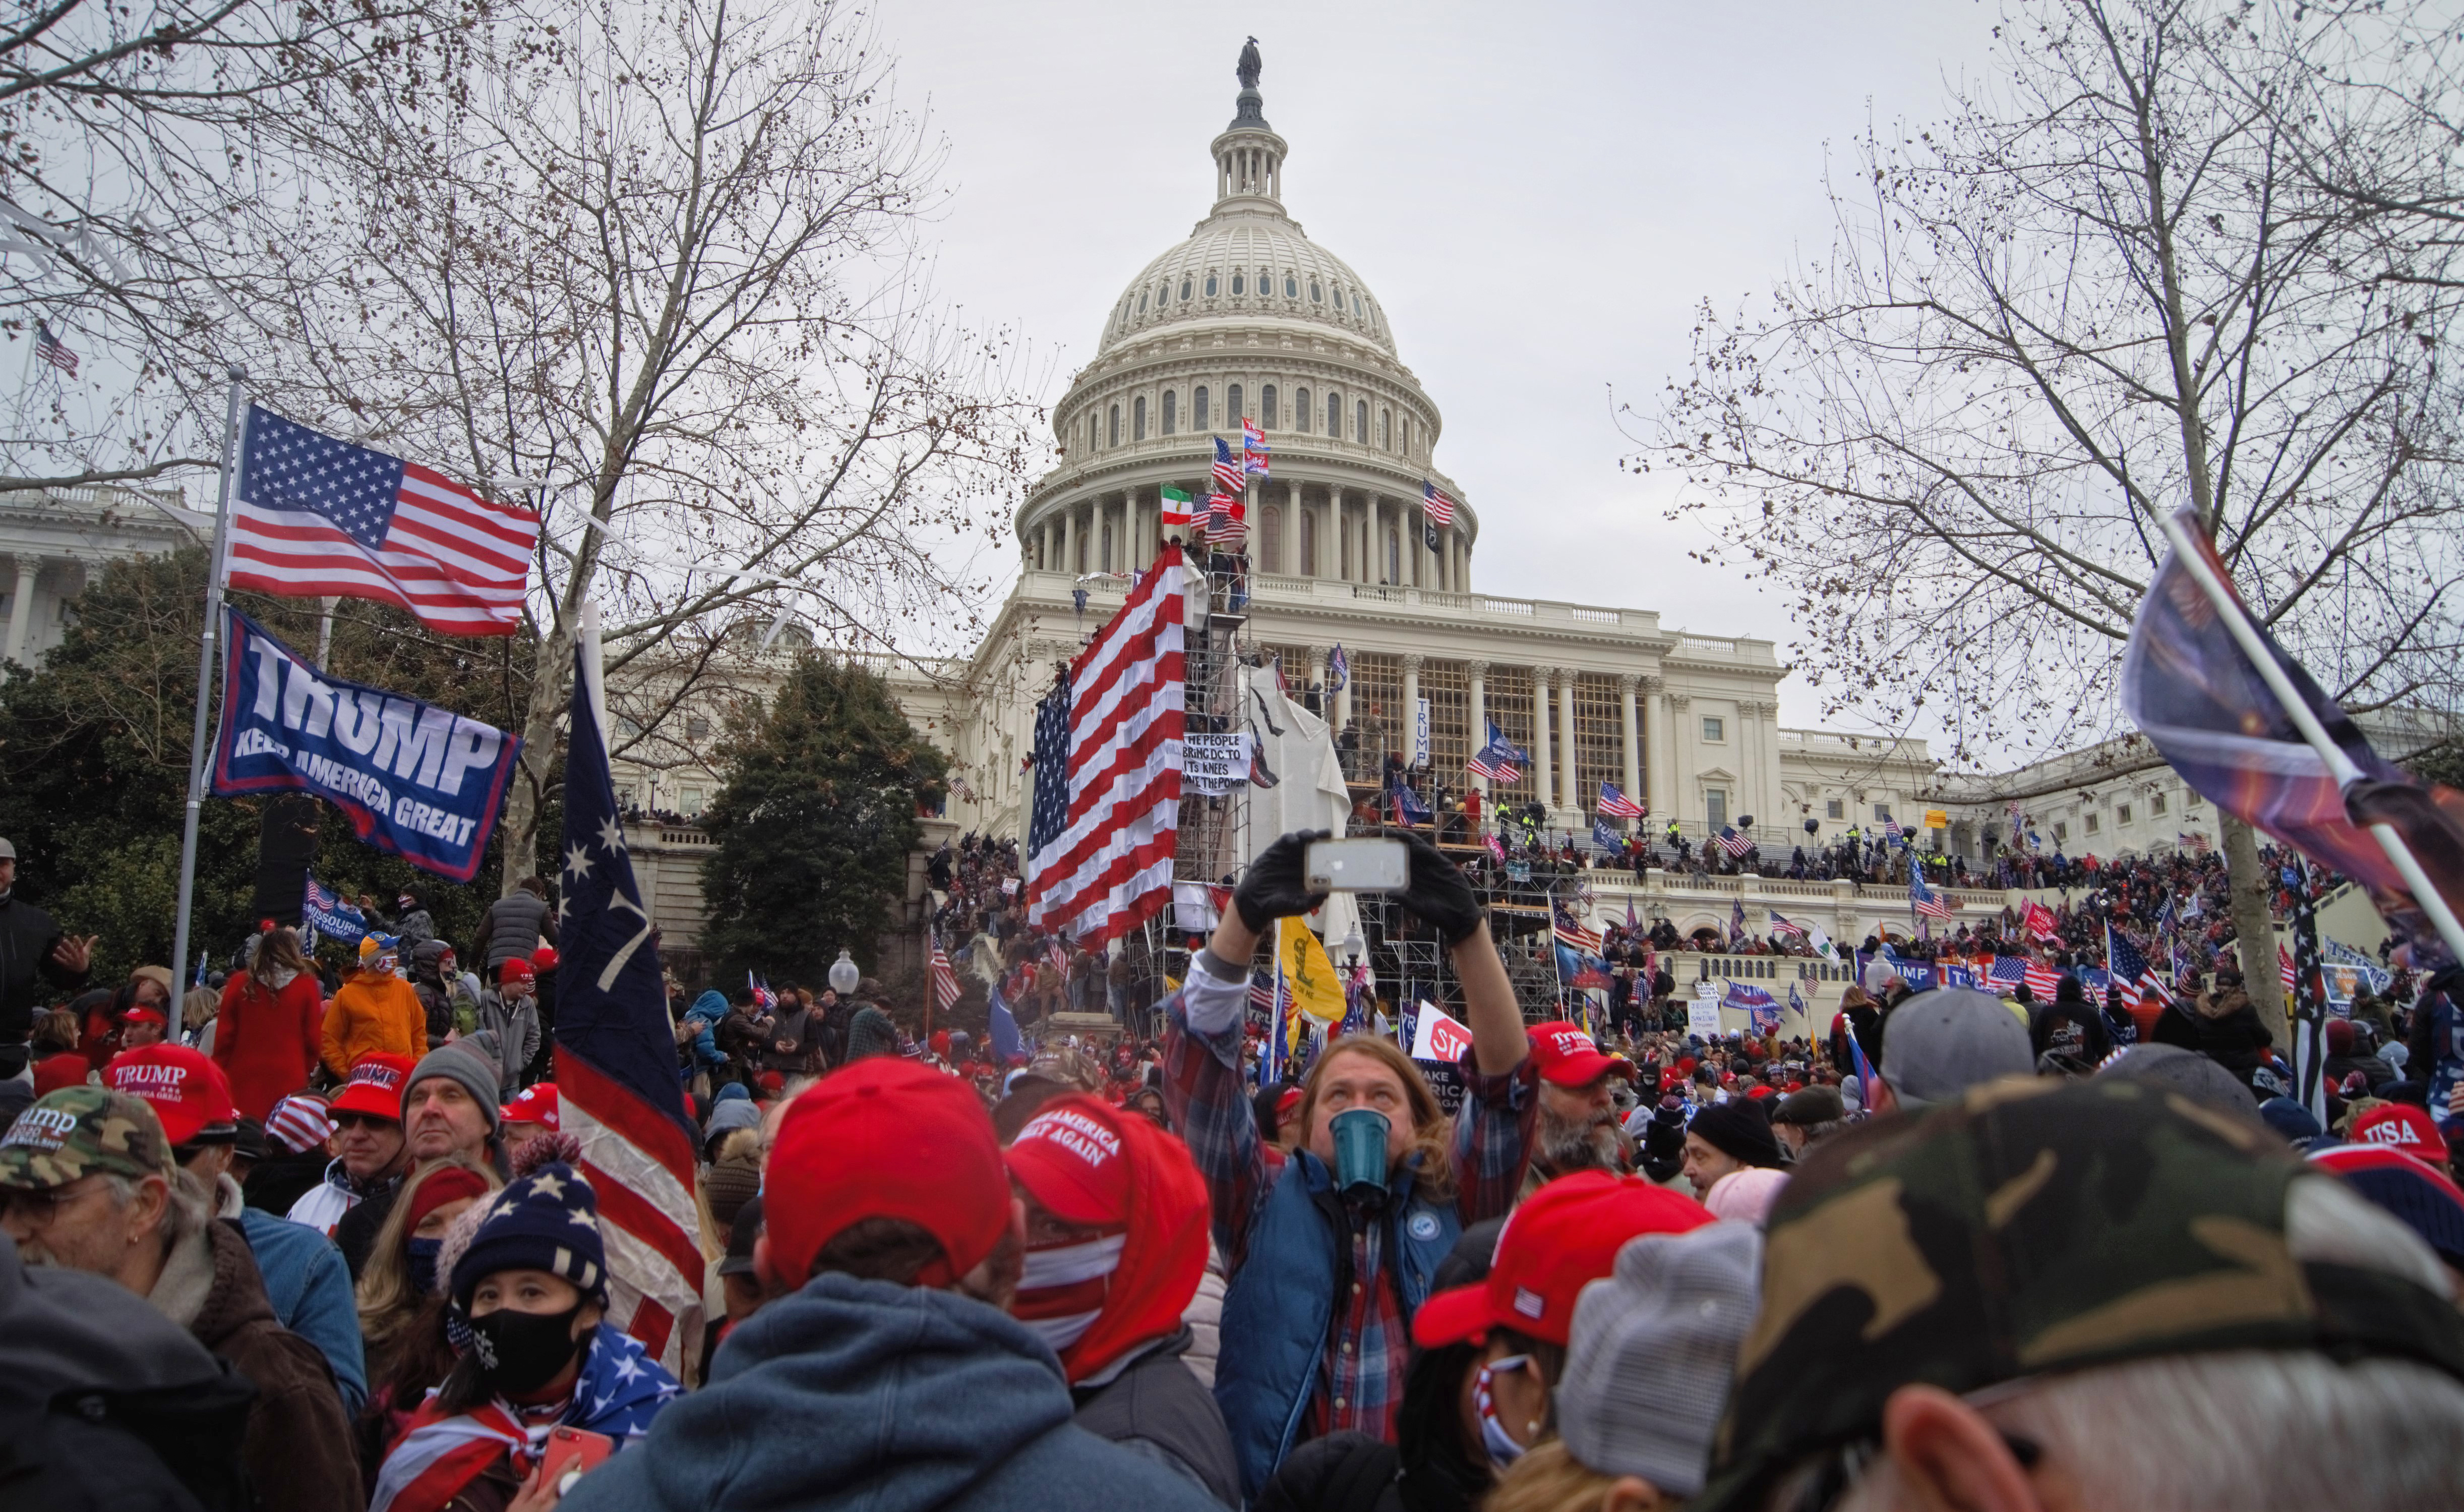
\includegraphics[width=0.6\linewidth]{jan6.jpg}
	\caption{A photo of the riot. By Tyler Merbler, CC--BY 2.0.}
\end{figure}
\end{frame}

% \appendix

\end{document}
